\iffalse 
\author{EE24BTECH11055}
\section{ce}
\chapter{2007}
\fi
%\begin{enumerate}[start=35]
		


	\item The right triangular truss is made of members having equal cross-sectional area of $1550\text{mm}^2$ and Young's modulus of $2 \times 10^5MPa$. The horizontal deflection of joint $Q$ is
		

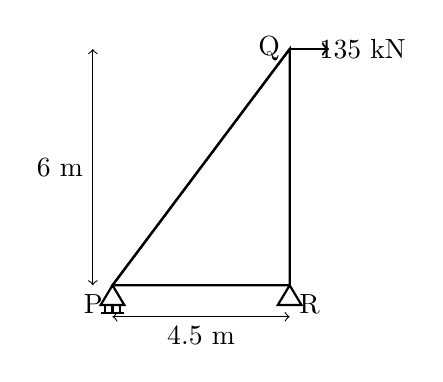
\begin{tikzpicture}[scale=0.5] 
   
    \coordinate (A) at (0,0);
    \coordinate (B) at (4.5,0);
    \coordinate (C) at (4.5,6);
    \node[below left] at (A) {P};
    \node[below right] at (B) {R};
    \node[left] at (C) {Q};
    \draw[thick] (A) -- (B) -- (C) -- cycle;
    \draw[thick] (A) -- (C);
    \draw[thick] (A) -- ++(-0.3,-0.5) -- ++(0.6,0) -- cycle;
    \draw[thick] (B) -- ++(-0.3,-0.5) -- ++(0.6,0) -- cycle;
    \draw[thick] (-0.3,-0.7) -- ++(0.6,0);
    \draw[thick] (-0.2,-0.7) -- (-0.2,-0.5);
     \draw[thick] (0.2,-0.7) -- (0.2,-0.5);
      \draw[thick] (0,-0.7) -- (0,-0.5);
    \draw[thick, ->] (C) -- ++(1,0) node[midway, right] {$135$ kN};
    \draw[<->] (A) ++(-0.5,0) -- ++(0,6) node[midway, left] {6 m};
    \draw[<->] (A) ++(0,-0.8) -- ++(4.5,0) node[midway, below] {4.5 m};
\end{tikzpicture}
	\begin{enumerate}
	\begin{multicols}{4}
		\item $2.47$ mm 
		\item $10.25$ mm
		\item $14.31$ mm
		\item $15.68$ mm
		\end{multicols}
	\end{enumerate}

\item The influence line diagram(ILD) shown is for the member 
\begin{center}
    

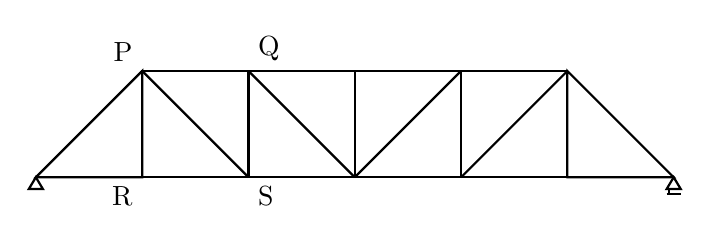
\begin{tikzpicture}[scale=0.3] 
    \coordinate (A) at (0,0);
    \coordinate (B) at (4.5,0);
    \coordinate (C) at (4.5,4.5);
    \coordinate (D) at (9,4.5);
    \coordinate (E) at (9,0);
    \coordinate (F) at (13.5,0);
    \coordinate (I) at (18,0);
    \coordinate (G) at (13.5,4.5);
    \coordinate (H) at (18,4.5);
    \coordinate (J) at (22.5,0);
    \coordinate (K) at (22.5,4.5);
    \coordinate (L) at (27,0);
    \node[above left] at (C) {P};
    \node[below left] at (B) {R};
    \node[above right] at (D) {Q};
    \node[below right] at (E) {S};
    \draw[thick] (A) -- (B) -- (C) -- cycle;
    \draw[thick] (E) -- (B) -- (C) -- (D) -- cycle;
    \draw[thick] (E) -- (F) -- (G) -- (D) -- cycle;
    \draw[thick] (G) -- (F) -- (I) -- (H) -- cycle;
    \draw[thick] (I) -- (H) -- (K) -- (J) -- cycle;
    \draw[thick] (K) -- (J) -- (L) -- cycle;
    \draw[thick] (A) -- (C);
    \draw[thick] (A) -- ++(-0.3,-0.5) -- ++(0.6,0) -- cycle;
    \draw[thick] (L) -- ++(-0.3,-0.5) -- ++(0.6,0) -- cycle;
    \draw[thick] (26.7,-0.7) -- ++(0.6,0);
    \draw[thick] (26.8,-0.7) -- (26.8,-0.5);
    \draw[thick] (26.8,-0.7) -- (26.8,-0.5);
    \draw[thick] (C) -- (E);
    \draw[thick] (D) -- (F);
    \draw[thick] (F) -- (H);
    \draw[thick] (I) -- (K);    
\end{tikzpicture}
\end{center}
\begin{center}
\begin{tikzpicture}[scale=0.3] 
    \coordinate (A) at (0,0);
    \coordinate (B) at (4.5,-2);
    % \coordinate (C) at (4.5,4.5);
    \coordinate (D) at (9,3);
    %\coordinate (E) at (9,0);
    %\coordinate (F) at (13.5,0);
    %\coordinate (I) at (18,0);
    %\coordinate (G) at (13.5,4.5);
    %\coordinate (H) at (18,4.5);
    %\coordinate (J) at (22.5,0);
    %\coordinate (K) at (22.5,4.5);
    %\coordinate (L) at (27,0);
    %\node[above left] at (C) {P};
    %\node[below left] at (B) {R};
    %\node[above right] at (D) {Q};
    %\node[below right] at (E) {S};
    \draw[thick] (A) -- (B) -- (D);
    \draw[thick] (D) -- (L) -- (A);
    %\draw[thick] (E) -- (F) -- (G) -- (D) -- cycle;
    %\draw[thick] (G) -- (F) -- (I) -- (H) -- cycle;
    %draw[thick] (I) -- (H) -- (K) -- (J) -- cycle;
   % \draw[thick] (K) -- (J) -- (L) -- cycle;
    %\draw[thick] (A) -- (C);
    %\draw[thick] (A) -- ++(-0.3,-0.5) -- ++(0.6,0) -- cycle;
    %\draw[thick] (L) -- ++(-0.3,-0.5) -- ++(0.6,0) -- cycle;
    %\draw[thick] (26.7,-0.7) -- ++(0.6,0);
    %\draw[thick] (26.8,-0.7) -- (26.8,-0.5);
    %\draw[thick] (26.8,-0.7) -- (26.8,-0.5);
    %\draw[thick] (C) -- (E);
    \draw[thick] (D) -- (9,0);
    \draw[thick] (B) -- (4.5,0);
    %\draw[thick] (I) -- (K);   
    \draw[thick] (2,-1.5) -- (3,-1);
    \node[below left] at (2,-1.5) {compression};
    \draw[->] (3,-1) -- (3.2,-0.8);
     \draw[thick] (10.5,3) -- (9.5,1);
    \node[above right] at (10.5,3) {tension};
    \draw[->] (9.5,1) -- (9.3,0.8);
    \node[below right] at (9,0) {IDL};
\end{tikzpicture}
\end{center}
	\begin{enumerate}
	\begin{multicols}{4}
		\item $PS$
		\item $RS$
		\item $PQ$
		\item $QS$
	\end{multicols}
	\end{enumerate}
\item Consider the following statements: \\
I. The compressive strength of concrete decreases with increase in water-cement ratio of the concrete mix.\\
II. Water is added to the concrete mix for hydration of cement and workability.\\
III. Creep and shrinkage of concrete are independent of the water-cement ratio in the concrete mix.\\
The TRUE statements are:

	\begin{enumerate}
		\begin{multicols}{4}
		\item I and II
		\item I, II and III
		\item II and III
		\item only II
			\end{multicols}
	\end{enumerate}
\item The percentage loss of prestress due to anchorage slip of $3mm$ in a concrete beam of length $30m$ which is post-tensioned by a tendon with an initial stress of $1200N/mm^2$ and modulus of elasticity equal to $2.1 X 10^5N/mm^2$ is: 
	\begin{enumerate}
			\begin{multicols}{4}
		\item $0.0175$
		\item $0.175$
		\item $1.75$
		\item $17.5$
			\end{multicols}
	\end{enumerate}
\item A concrete beam of rectangular cross-section of size $120$ $mm$ (width) and $200$ $mm$ (depth) is prestressed by a straight tendon to an effective force of $150$ $kN$ at an eccentricity of $20$ $mm$ (below the centroidal axis in the depth direction). The stresses at the top and bottom fibres of the section are:
	\begin{enumerate} 
			\item $2.5 N/mm^2$(compression), $10 N/mm^2$(compression)
			\item $10 N/mm^2$(tension), $2.5 N/mm^2$(compression)
			\item $3.75 N/mm^2$(tension), $3.75 N/mm^2$(compression)
			\item $2.75 N/mm^2$(compression), $3.75 N/mm^2$(compression)
			\end{enumerate}
\item Consider the following statements:\\
I. Modulus of elasticity of concrete increases with increase in compressive strength of concrete.\\
II. Brittleness of concrete increases with decrease in compressive strength of concrete.\\
III. Shear strength of concrete increases with increase in compressive strength of concrete.\\
The TRUE statements are:
	\begin{enumerate}
		\begin{multicols}{4}
		\item II and III
		\item I, II and III
		\item I and II
		\item I and III
		\end{multicols}
	\end{enumerate}
 %41
\item  A steel flat of rectangular section of size $70 \times 6$ $mm$ is connected to a gusset plate by three bolts each having a shear capacity of $15$ $kN$ in holes having diameter $11.5$ $mm$. If the allowable tensile stress in the flat is $150$ $MPa$, the maximum tension that can be applied to the flat is:\\
\begin{center}
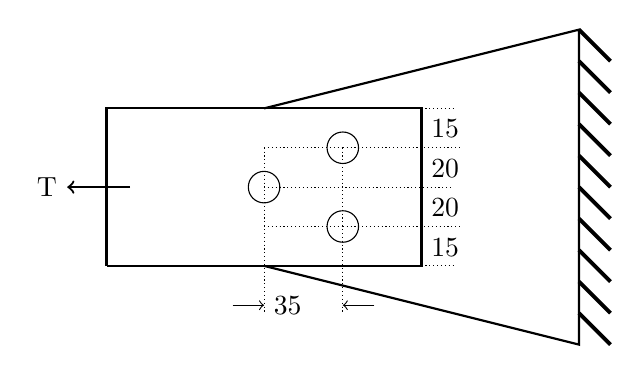
\begin{tikzpicture}
   \coordinate (A) at (0,0);
   \coordinate (B) at (4,0);
   \coordinate (C) at (4,2);
   \coordinate (D) at (0,2);
   \coordinate (E) at (6,3);
   \coordinate (F) at (6,-1);
   \draw[thick] (A) -- (B) -- (C) -- (D) -- (A);
   \draw[thick] (2,2) -- (6,3) -- (6,-1) -- (2,0);
   \draw[densely dotted] (3,1.5) -- (4.5,1.5);
   \draw[densely dotted] (2,1) -- (4.4,1);
   \draw[densely dotted] (3,0.5) -- (4.5,0.5);
   \draw[densely dotted] (4,2) -- (4.4,2);
   \draw[densely dotted] (4,0) -- (4.4,0);
   \draw[densely dotted] (3,1.5) -- (3,-0.6);
   \draw[densely dotted] (2,1.5) -- (3,1.5);
   \draw[densely dotted] (2,0.5) -- (3,0.5);
   \draw[densely dotted] (2,1.5) -- (2,-0.6);
   \draw (3,1.5) circle (0.2cm);
   \draw (3,0.5) circle (0.2cm);
   \draw (2,1) circle (0.2cm);
   \draw[->] (1.6,-0.5) -- (2,-0.5) node[right] {35};
   \draw[->] (3.4,-0.5) -- (3,-0.5);
   \draw[->,thick] (0.3,1) -- (-0.5,1) node[left] {T};
   \node[above right] at (4,1.5) {15};
   \node[above right] at (4,1) {20};
   \node[above right] at (4,0.5) {20};
   \node[above right] at (4,0) {15};
   \draw[line width=0.5mm] (6,3) -- (6.4,2.6);
   \draw[line width=0.5mm] (6,2.6) -- (6.4,2.2);
   \draw[line width=0.5mm] (6,2.2) -- (6.4,1.8);
   \draw[line width=0.5mm] (6,1.8) -- (6.4,1.4);
   \draw[line width=0.5mm] (6,1.4) -- (6.4,1.0);
   \draw[line width=0.5mm] (6,1.0) -- (6.4,0.6);
   \draw[line width=0.5mm] (6,0.6) -- (6.4,0.2);
   \draw[line width=0.5mm] (6,0.2) -- (6.4,-0.2);
   \draw[line width=0.5mm] (6,-0.2) -- (6.4,-0.6);
   \draw[line width=0.5mm] (6,-0.6) -- (6.4,-1);
\end{tikzpicture}
\end{center}
	\begin{enumerate}
	\begin{multicols}{4}
		\item $42.3kN$
		\item $52.65kN$
		\item $59.5kN$
		\item $63.0kN$
	\end{multicols}
	\end{enumerate}
\item  A bracket connection is made with four bolts of $10mm$ diameter and supports a load of $10kN$ at an eccentricity of $100mm$. The maximum force to be resisted by any bolt will be:\\
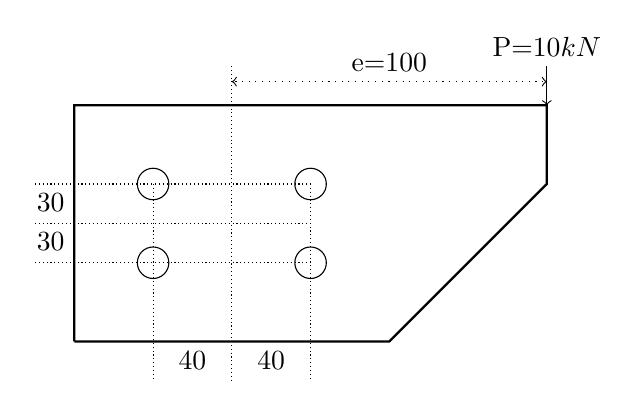
\begin{tikzpicture}
  \coordinate (A) at (0,0);
  \coordinate (B) at (4,0);
  \coordinate (C) at (6,2);
  \coordinate (D) at (6,3);
  \coordinate (E) at (0,3);
  \coordinate (F) at (3,2);
  \coordinate (G) at (1,1);
  \coordinate (H) at (3,1);
  \coordinate (I) at (1,2);
  \draw[thick] (A) -- (B) -- (C) -- (D) -- (E) -- (A);
  \draw[densely dotted] (-0.5,2) -- (F);
  \draw[densely dotted] (-0.5,1.5) -- (3,1.5);
  \draw[densely dotted] (-0.5,1) -- (H);
  \draw[densely dotted] (I) -- (1,-0.5);
  \draw[densely dotted] (F) -- (3,-0.5);
  \draw[densely dotted] (2,3.5) -- (2,-0.5);
  \draw[->] (6,3.5) -- (6,3) ;
  \node[above] at (6,3.5) {P=$10kN$};
  \node[below left] at (0,2) {30};
  \node[below left] at (0,1.5) {30};
  \node[below] at (1.5,0) {40};
  \node[below] at (2.5,0) {40};
  \draw (I) circle (0.2cm);
  \draw (F) circle (0.2cm);
  \draw (G) circle (0.2cm);
  \draw (H) circle (0.2cm);
  \draw[->, dotted] (4,3.3) -- (6,3.3) ;
  \draw[->,dotted] (4,3.3) -- (2,3.3) ;
  \node[above] at (4,3.3) {e=100};
\end{tikzpicture}
        \begin{enumerate} 
	\begin{multicols}{4}
		\item $5kN$
		\item $6.5kN$
		\item $6.8kN$
		\item $7.16kN$
	\end{multicols}
	\end{enumerate}
\item The plastic collapse load $W_p$ for the propped cantilever supporting two point loads as shown in figure in terms of plastic moment capacity, $M_p$, is given by:
\begin{center}
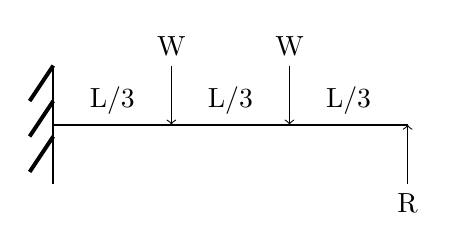
\begin{tikzpicture}[scale=1.5]
    \draw[thick] (0,0) -- (1,0) -- (2,0) -- (3,0);
    \draw[->] (1,0.5) -- (1,0) ;
    \draw[->] (2,0.5) -- (2,0) ;
    \draw[-> ] (3,-0.5) -- (3,0) ;
    \draw[thick] (0,-0.5) -- (0,0.5);
    \node[above] at (1,0.5) {W};
    \node[above] at (2,0.5) {W};
    \node[below] at (3,-0.5) {R};
    \node[above] at (0.5,0) {L/3};
    \node[above] at (1.5,0) {L/3};
    \node[above] at (2.5,0) {L/3};
    \draw[line width=0.5mm] (0,0.5) -- (-0.2,0.2);
    \draw[line width=0.5mm] (0,0.2) -- (-0.2,-0.1);
    \draw[line width=0.5mm] (0,-0.1) -- (-0.2,-0.4);
\end{tikzpicture}
\end{center}
	\begin{enumerate}
	\begin{multicols}{4}
			
		\item $3M_p/L$
		\item $4M_p/L$
		\item $5M_p/L$
		\item $6M_p/L$
		\end{multicols}
			
	\end{enumerate}
\item Sieve analysis on a dry soil sample of mass $1000g$ showed that $980g$ and $270g$ of soil pass through $4.75mm$ and $0.075mm$ sieve, respectively. The liquid limit and plastic limits of the soil fraction passing through $425\mu$ sieves are $40\%$ and  $18\%$, respectively. The soil may be classified as:
	\begin{enumerate}
	\begin{multicols}{4}		
		\item SC
		\item MI
		\item CI
		\item SM
	\end{multicols}
	\end{enumerate}
\item The water content of a saturated soil and the specific gravity of soil solids were found to be $30\%$ and $2.70$ respectively. Assuming the unit weight of water to be $10kN/m^3$, the saturated unit weight($kN/m^3$) and the void ratio of the soil are: 
	\begin{enumerate}
		\begin{multicols}{4}
		\item $19.4, 0.81$
		\item $18.5, 0.30$
		\item $19.4, 0.45$
		\item $18.5, 0.45$
			\end{multicols}
	\end{enumerate}
\item The factor of safety of an infinite soil slope shown in the figure having the properties $c=0, \phi= 35^\circ,\gamma_{\text{dry}}=16kN/mm^3$ and $\gamma_{\text{sat}}=20kN/m^3$ is approximately equal to:   \\
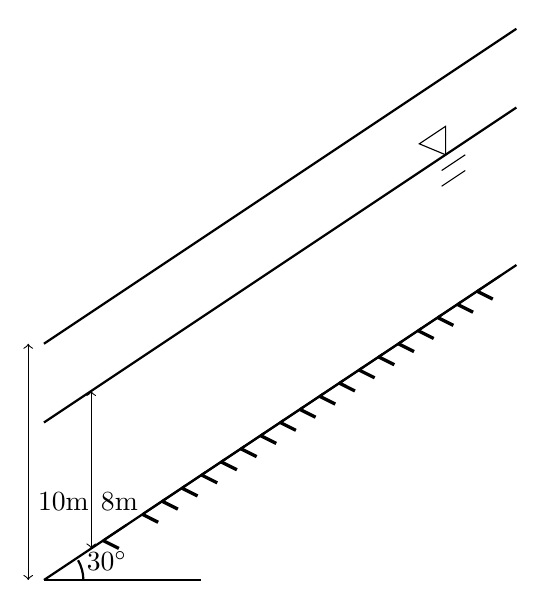
\begin{tikzpicture}
   \draw[thick] (0,0) -- (6,4) ;
   \draw[thick] (0,2) -- (6,6) ;
   \draw[thick] (0,3) -- (6,7) ;
   \draw[thick] (0,0) -- (2,0) ;
   \draw[<->] (-0.2,0) -- (-0.2,3) ;
   \draw[<->] (0.6,0.4) -- (0.6,2.4) ;
   \node[right] at (0.6,1) {8m};
   \node[right] at (-0.2,1) {10m};
   \begin{scope}[shift={(5.1, 5.4)}, rotate=33.69] 
       \draw[black] (0,0) -- ++(-0.2, 0.3) -- ++(0.4, 0) -- cycle;
   \end{scope}
    \draw (5.05, 5.2) -- ++(0.3, 0.2); 
   \draw (5.05, 5.0) -- ++(0.3, 0.2);
    \draw[thick] (0.5,0) arc[start angle=0,end angle=30,radius=0.5cm];
    \node[above ] at (0.8,0) {$30^\circ$};
    \foreach \x in {0.751,1.25, 1.5,1.75,2,2.25,2.5,2.75, 3,3.25,3.5,3.75, 4,4.25,4.5,4.75, 5,5.25,5.5} {
       \draw[very thick] (\x, \x * 2/3) -- ++(0.2, -0.1);
       \draw[thick] (\x, \x * 2/3) -- ++(0.3, 0.2);
   }
\end{tikzpicture}

	\begin{enumerate}
		\item $0.70$
		\item $0.80$
		\item $1.00$
		\item $1.20$		
	\end{enumerate}
\item Match the following groups.\\
\begin{center}
\begin{tabular}{ll}
    {Group-I} & {Group-II} \\
    P. Constant head permeability test & 1. Pile foundations \\
    Q. Consolidation test & 2. Specific gravity \\
    R. Pycnometer test & 3. Clay soil \\
    S. Negative skin friction & 4. Sand \\
\end{tabular}
\end{center}
	\begin{enumerate}
			%\begin{multicols}{2}
		\item P-$4$, Q-$3$, R=$2$, S=$1$
		\item P-$4$, Q-$2$, R=$3$, S=$1$
		\item P-$3$, Q-$4$, R=$2$, S=$1$
		\item P-$4$, Q-$1$, R=$2$, S=$3$
			%\end{multicols}
	\end{enumerate}
\item The bearing capacity of a rectangular footing of plan dimensions $1.5$ m X $3$ m resting on the surface of a sand deposit was estimated as $600kN/m^2$ when the water table is far below the base of the footing. The bearing capacities in $kN/m^2$ when the water level rises to depths of $3m$, $1.5m$ and $0.5m$ below the base of the footing are:
	\begin{enumerate} 
			\begin{multicols}{4}	
		\item $600,600,400$
		\item $600,450,350$
		\item $600,500,250$
		\item $600,400,250$
			\end{multicols}
	\end{enumerate}
\item What is the ultimate capacity in $kN$ of the pile group shown in the figure assuming the group to fail as a single block?\\
\begin{center}
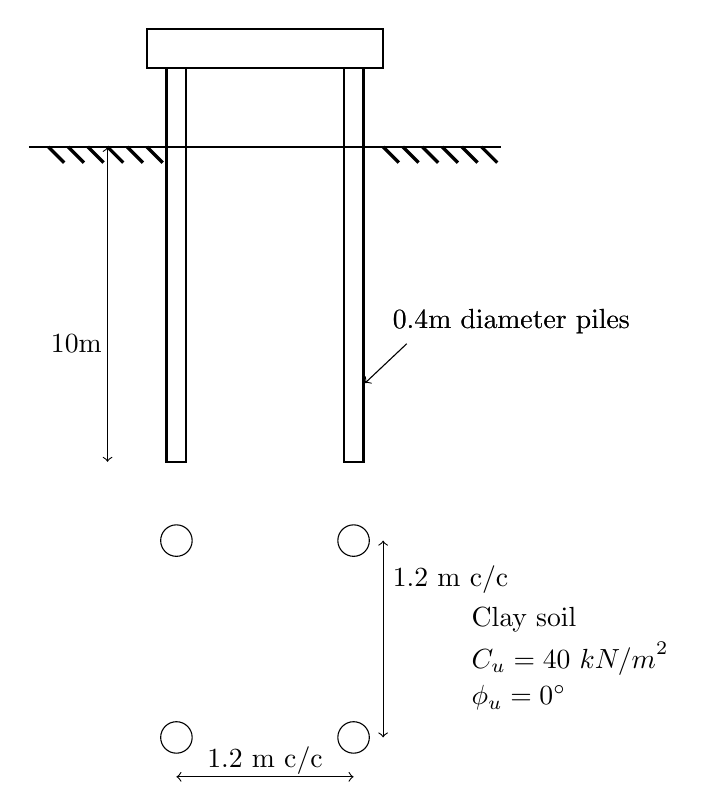
\begin{tikzpicture}
    \draw[thick] (-1.25,1) -- (-1.25,-4) -- (-1,-4) -- (-1,1);
    \draw[thick] (1.25,1) -- (1.25,-4) -- (1,-4) -- (1,1);
    \draw[thick] (-1.5,1) -- (-1.5,1.5) -- (1.5,1.5) -- (1.5,1)-- cycle;
    \draw[thick] (-3,0) -- (3,0);
    \draw[<->] (-2,-4) -- (-2,0);
    \draw[<->] (1.125,-8) -- (-1.125,-8);
    \draw[<->] (1.5,-5)--(1.5,-7.5);
    \draw (1.125,-5) circle (0.2cm);
    \draw (1.125,-7.5) circle (0.2cm);
    \draw (-1.125,-5) circle (0.2cm);
    \draw (-1.125,-7.5) circle (0.2cm);
    \draw[->] (1.8,-2.5) -- (1.27,-3);
    \node[above right] at (1.5,-2.5) {0.4m diameter piles};
    \node[left] at (-1.95,-2.5) {10m};
    \node[above right] at (1.5,-2.5) {0.4m diameter piles};
    \node[right] at (1.5,-5.5) {1.2 m c/c};
    \node[below] at (0,-7.5) {1.2 m c/c};
    \foreach \x in {-2.75,-2.5,-2.25, -2,-1.75, -1.5,  1.5,1.75, 2,2.25, 2.5,2.75} {
       \draw[very thick] (\x, 0) -- ++(0.2, -0.2); 
   }
   \node[right] at (2.5,-6) {Clay soil};
   \node[right] at (2.5,-6.5) {$\text{C}_u=40$ $\text{kN/m}^2$}; 
   \node[right] at (2.5,-7) {$\phi_u=0^{\circ}$};
\end{tikzpicture}
\end{center}
	\begin{enumerate}
			\begin{multicols}{4}
		\item $921.6$
		\item $1177.6$
		\item $2438.6$
		\item $3481.6$
			\end{multicols}
	\end{enumerate}
\item A horizontal water jet with a velocity of $10m/s$ and cross sectional area of $10\text{mm}^2$ strikes a flat plate held normal to the flow direction. The density of water is $1000\text{kg/m}^3$. The total force on the plate due to the jet is
	\begin{enumerate}
			\begin{multicols}{4}
		\item $100$ N
		\item $10$ N
		\item $1$ N
		\item $0.1$ N
			\end{multicols}
	\end{enumerate}
\item A $1:50$ scale model of a spillway is to be tested in the laboratory. The discharge in the prototype is $1000m^3/s$. The discharge to be maintained in the model test is: 
	\begin{enumerate}
			\begin{multicols}{4}
		\item $0.057m^3/s$ 
		\item $0.08m^3/s$
		\item $0.57m^3/s$
		\item $5.7m^3/s$
			\end{multicols}
	\end{enumerate}
%\end{enumerate}
